\section[Intro]{Introduction}
\begin{frame}{\textbf{G}lobal \textbf{N}avigation \textbf{S}atellite \textbf{S}ystem}
    \begin{itemize}
        \item \textbf{GNSS} has been successfully applied in many fields:
    \end{itemize}

    \begin{figure}[!htb]
        \centering
        \begin{subfigure}[b]{0.3\textwidth}
            \centering
            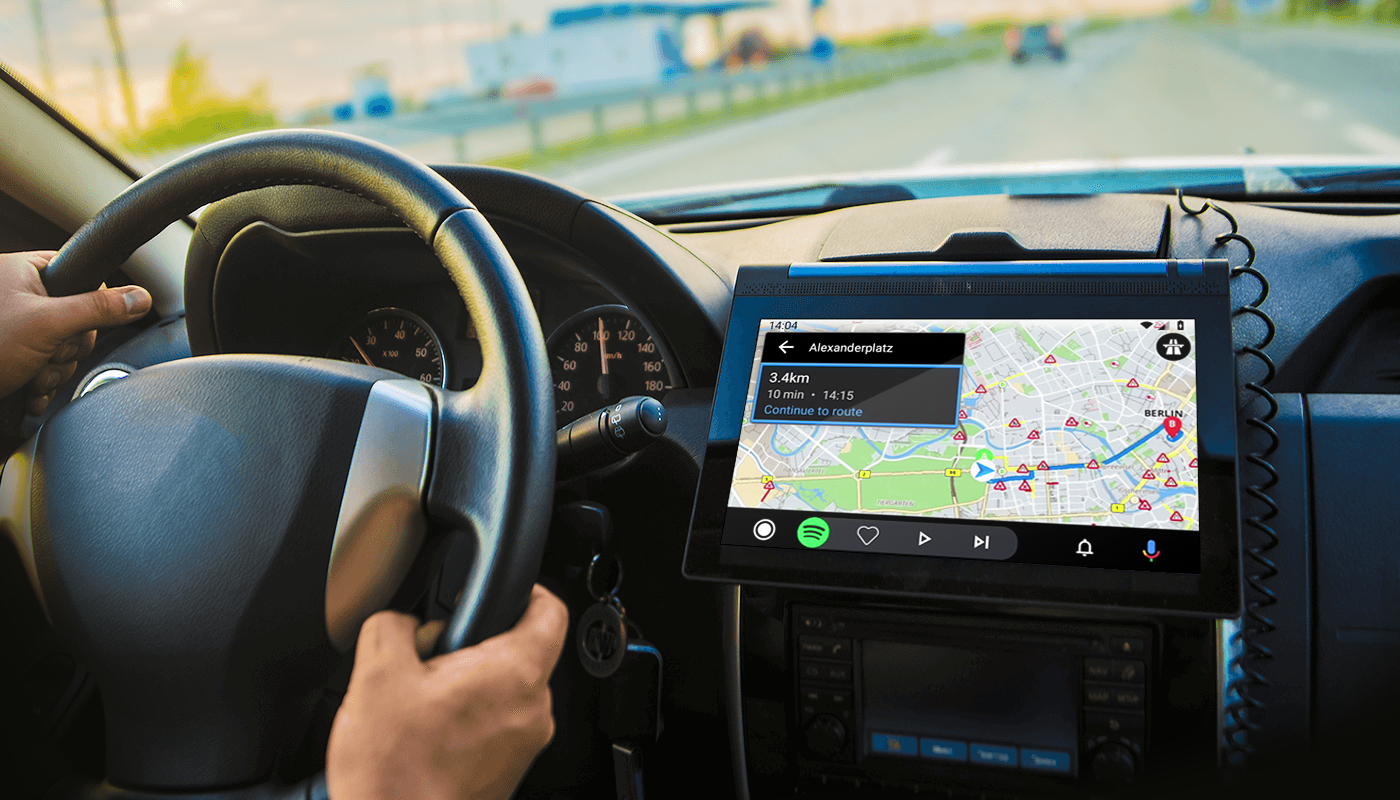
\includegraphics[width=\linewidth]{images/carnav.png}
            \caption{Car navigation}
            \label{fig:carnav}
        \end{subfigure}
        \hfill
        \begin{subfigure}[b]{0.3\textwidth}
            \centering
            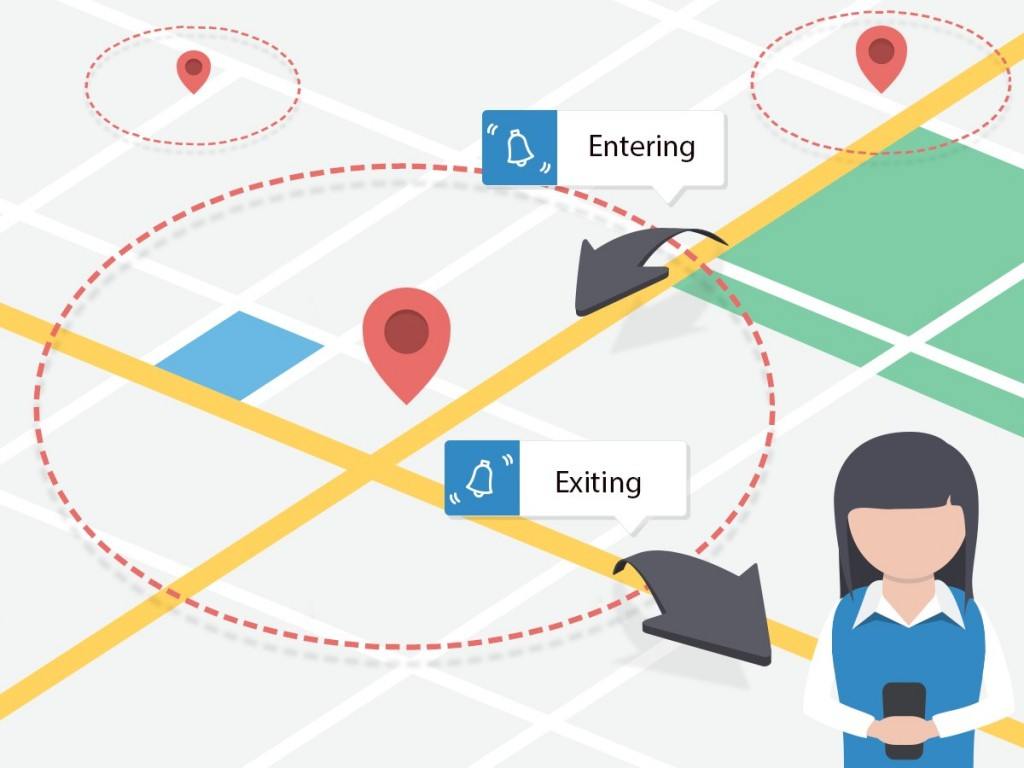
\includegraphics[width=\linewidth]{images/geofencing.jpg}
            \caption{Geofencing}
            \label{fig:geofencing}
        \end{subfigure}
        \hfill
        \begin{subfigure}[b]{0.3\textwidth}
            \centering
            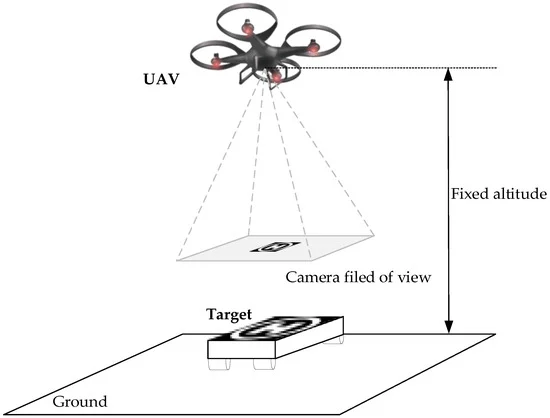
\includegraphics[width=\linewidth]{images/target.jpg}
            \caption{Target tracking}
            \label{fig:target}
        \end{subfigure}
           \caption{Some examples of application}
           \label{gnss}
    \end{figure}

    \begin{itemize}   
        \item It's \textbf{difficult to use} for inside location: \textbf{signal} is \textit{blocked} by buildings, trees, obstacles, ...
    \end{itemize}
\end{frame}

\begin{frame}{Indoor localization}
    \begin{itemize}
        \item It's even more \textbf{challenging}:
            \begin{itemize}
                \item Indoor spaces are more \textbf{complicated} in terms of \textit{layout}, \textit{topology}, \textit{space constraint};\item Indoor applications need more \textbf{accuracy}.
            \end{itemize}
        \item Multiple systems have been proposed in recent years:
        \end{itemize}
    
        \begin{figure}[!htb]
            \centering
            \begin{subfigure}[t]{0.24\textwidth}
                \centering
                
\includegraphics[width=\linewidth]{images/wifi.png}
                \caption{WiFi}
                \label{fig:wifi}
            \end{subfigure}
            \hfill
            \begin{subfigure}[t]{0.24\textwidth}
                \centering
                
\includegraphics[width=\linewidth]{images/zigbee.png}
                \caption{Zigbee}
                \label{fig:zigbee}
            \end{subfigure}
            \hfill
            \begin{subfigure}[t]{0.24\textwidth}
                \centering
                
\includegraphics[width=\linewidth]{images/bluetooth.png}
                \caption{Bluetooth}
                \label{fig:bluetooth}
            \end{subfigure}
            \hfill
            \begin{subfigure}[t]{0.24\textwidth}
                \centering
                
\includegraphics[width=\linewidth]{images/uwb.jpg}
                \caption{Ultra-wideband}
                \label{fig:uwb}
            \end{subfigure}
               \caption{Some examples of indoor localization systems}
               \label{indoor}
        \end{figure}
    
        \begin{itemize}
        \item Each technique has \textbf{drawbacks} in terms of accuracy, cost coverage, complexity and applicability.
    \end{itemize}
\end{frame}

\begin{frame}{Landmark}
    \begin{block}{Landmark for \textbf{Indoor Localization}}
        A landmark is a \textbf{spatial constraint}.\\
        It's a location point where \textit{at least one sensor} shows a \textbf{distinctive}, \textbf{stable}, and \textbf{identifiable pattern}.
    \end{block}
    
    \greent{Advantages}
    \begin{itemize}
        \item \textbf{Naturally distributed} location points in indoor environments;
        \item \textbf{Easy to bound} the localization \textbf{error} with no extra cost.
    \end{itemize}
    
    \redt{Disadvantages}
    \begin{itemize}
        \item \textbf{Economically} and \textbf{computationally expensive} systems;
        \item \textbf{Performance} depends on \textbf{completeness of landmarks}.
    \end{itemize}
    
\end{frame}

\begin{frame}{LG-Loc}
    \begin{block}{Landmark-Guided Localization}
        It's a novel \textbf{graph-based indoor localization} method for smartphones
    \end{block}

    Compared with existing landmark-based localization methods:
    \begin{itemize}
        \item Computationally \textbf{efficient};
        \item Handles \textbf{incomplete landmarks}.
    \end{itemize}

    \begin{block}{Landmark graph}
        It's a \textbf{directed graph} where nodes are landmarks and edges are accessible paths with heading information
    \end{block}
\end{frame}

\begin{frame}{LG-Loc $\sim$ Phases \& Challenges}
    This method consists of two \textbf{phases:}
    \begin{enumerate}
        \item \textit{Offline:}
        \begin{itemize}
            \item \textbf{Collect data} from several \textbf{smartphone sensors};
            \item \textbf{Construct} the \textbf{initial landmark graph} and \textbf{update it} with more landmarks.
        \end{itemize}
        \item \textit{Online:}
        \begin{itemize}
            \item Use newly collected data for \textbf{location initialization}, \textbf{estimation}, and \textbf{calibration}.
        \end{itemize}
    \end{enumerate}

    \textbf{Challenges:}
    \begin{enumerate}
        \item Infer the \textbf{initial location} without \textbf{manual input}.
        \item \textbf{Recognize} landmarks \textbf{effectively}.
        \item Handle \textbf{missing landmarks}.
    \end{enumerate}
\end{frame}